%\documentclass[10pt,preprint,nocopyrightspace,nonatbib]{sigplanconf}
%\documentclass[9pt,preprint]{sig-alternate-no-permission}
%\documentclass[9pt,preprint]{sig-alternate}
\documentclass[letterpaper,twocolumn,10pt]{article}
%\usepackage{usenix}
%\documentclass[pageno]{jpaper}
%\documentclass[10pt,preprint]{sigplanconf}
%\documentclass[sigplan,10pt,anonymous]{acmart}\settopmatter{printfolios=true}
%\documentclass[10pt,conference]{IEEEtran}
\usepackage{usenix2019_v3}
\usepackage{mathptmx} % This is Times font

% The following \documentclass options may be useful:

% preprint      Remove this option only once the paper is in final form.
% 10pt          To set in 10-point type instead of 9-point.
% 11pt          To set in 11-point type instead of 9-point.
% authoryear    To obtain author/year citation style instead of numeric.

\usepackage{minted}
\usepackage{epsfig}
%\usepackage[utf8x]{inputenc}
\usepackage{algorithm}
\usepackage{amsmath, amssymb}
\usepackage[noend]{algpseudocode}
\usepackage{enumitem}      % adjust spacing in enums
%\usepackage{subfig}
\usepackage{caption}
\usepackage{subcaption}
\usepackage{multirow}
\usepackage{rotating}
\usepackage{wrapfig}
\usepackage{tabu}
\usepackage{pifont}
\usepackage[normalem]{ulem}

\let\bibhang\relax
\let\citename\relax
\let\bibfont\relax
\let\citeauthor\relax
\let\Citeauthor\relax
\let\citefullauthor\relax
\let\citetext\relax
\let\defcitealias\relax
\let\citet\relax
\let\citep\relax
\let\Citep\relax
\let\Citealt\relax
\let\citealt\relax
\let\citealp\relax
\let\Citealp\relax
\let\Citet\relax

\expandafter\let\csname ver@natbib.sty\endcsname\relax

\DeclareCaptionFormat{subfig}{\figurename~#1#2#3}
\DeclareCaptionSubType*{figure}
%\captionsetup[subfigure]{format=subfig,labelsep=colon,labelformat=simple}

\usepackage[natbib=true,backend=bibtex,firstinits=true,style=numeric-comp,sorting=nyt,defernumbers,maxnames=99,maxcitenames=99]{biblatex}
\usepackage{balance}
\usepackage{adjustbox}

\usepackage{pgfplots}
% options for pgfplots
\pgfplotsset{compat=1.8,compat/show suggested version=false}
\usetikzlibrary{plotmarks}
\usetikzlibrary{calc}
%\pgfplotsset{compat=newest}
\pgfplotsset{
   /pgfplots/bar  cycle  list/.style={/pgfplots/cycle  list={%
        {black,fill=black!30!white,mark=none},%
        {black,fill=red!30!white,mark=none},%
        {black,fill=green!30!white,mark=none},%
        {black,fill=yellow!30!white,mark=none},%
        {black,fill=brown!30!white,mark=none},%
     }
   },
}
% begin of externalization
\usetikzlibrary{external}
\tikzexternalize[prefix=out/]
\tikzexternalize
% don't externalize todonotes
%\makeatletter
%\renewcommand{\todo}[2][]{\tikzexternaldisable\@todo[#1]{#2}\tikzexternalenable}
%\makeatother
% end of externalization
\usetikzlibrary{patterns}
\usepgfplotslibrary{groupplots}
\pgfplotsset{
every axis label/.append style={font=\small},
tick label style={font=\small},
}
% options for paragraphs and lists
\setlist{noitemsep,topsep=0pt}
% options for biblatex
\bibliography{refs}
%\renewcommand{\bibfont}{\footnotesize}


\usepackage{fancyhdr}

% Ensure letter paper
\pdfpagewidth=8.5in
\pdfpageheight=11in

\fancypagestyle{firstpage}{
%   \fancyhf{}
% \setlength{\headheight}{50pt}
% \renewcommand{\headrulewidth}{0pt}
%   \fancyhead[C]{\normalsize{CONFIDENTIAL DRAFT --- DO NOT DISTRIBUTE}}
%   \pagenumbering{arabic}
}

\pagenumbering{arabic}


\setlength{\itemsep}{0pt}
%\setlength{\topsep}{0pt}
%\setlength{\partopsep}{0pt}
%\setlength{\parsep}{1pt}
%\setlength{\parskip}{1pt}
\setlength{\abovecaptionskip}{1pt plus 2pt minus 2pt}
\setlength{\textfloatsep}{5pt}
%\setlength{\bibitemsep}{0pt}

\sloppy

\newif{\ifanonymous}
\anonymoustrue

%\newcommand{\comment}[[1]{\textcolor{red}{#1}}
\newcommand{\myworries}[1]{\textcolor{red}{#1}}
\newcommand{\cutout}[1]{}
\newcommand{\smallcaption}[1]{\caption[#1]{{\protect\small \protect\bf #1}}}
\newcommand{\dids}{{\sc dids}}

\graphicspath{{./figs/}}
\date{}

\algnewcommand{\LineComment}[1]{\(\triangleright\) #1}

% some useful shortcuts
\newcommand{\ie}{\textit{i.e., }}
\newcommand{\eg}{\textit{e.g., }}
\newcommand{\CC}{C\nolinebreak\hspace{-.05em}\raisebox{.5ex}{\tiny\bf +}\nolinebreak\hspace{-.10em}\raisebox{.5ex}{\tiny\bf +}}

% units for results
\newcommand{\us}{\,$\mu$s}
\newcommand{\ms}{\,ms}
\newcommand{\KB}{\,KB}
\newcommand{\MB}{\,MB}
\newcommand{\GB}{\,GB}
\newcommand{\MHz}{\,MHz}
\newcommand{\GHz}{\,GHz}

% new latex commands:
%   Remove long section
\newcommand{\PUNT}[1]{}
\newcommand{\TABLETWO}[1]{}
%   Label work to be done
\definecolor{gray}{gray}{0.75}
\newcommand{\TODO}[1]{\textcolor{gray}{\textbf{\ [TODO:\ #1]\ }}}
\newcommand{\TR}[1]{#1}
%\newcommand{\TR}[1]{}
%\newcommand{\TODO}[1]{}
\newcommand{\FIX}[1] {\textcolor{red}{\textbf{\ [FIX:\ #1]\ }}}
%   Referencing various pieces of the document:
\newcommand{\figref}[1]{Fig.~\ref{fig:#1}}
\newcommand{\figsref}[2]{Figures~\ref{fig:#1} and~\ref{fig:#2}}
\newcommand{\figrref}[2]{Figures~\ref{fig:#1}--\ref{fig:#2}}
\newcommand{\secref}[1]{Section~\ref{sec:#1}}
\newcommand{\secsref}[2]{Sections~\ref{sec:#1} and~\ref{sec:#2}}
\newcommand{\eqnref}[1]{Eqn.~\ref{eqn:#1}}
\newcommand{\eqnsref}[2]{Equations~\ref{eqn:#1} and~\ref{eqn:#2}}
\newcommand{\eqnrref}[2]{Equations~\ref{eqn:#1}--\ref{eqn:#2}}
\newcommand{\insref}[1]{Instruction~\ref{ins:#1}}
\newcommand{\tblref}[1]{Table~\ref{tbl:#1}}
\newcommand{\appref}[1]{Appendix~\ref{app:#1}}

\newcommand{\algoref}[1]{Algorithm~\ref{algo:#1}}

% Custom hyphenation rules

%\DeclareMathOperator{\minimize}{minimize}
%\DeclareMathOperator{\st}{s.t.}
%\DeclareMathOperator*{\argmin}{arg\,min}
%\DeclareMathOperator*{\argmax}{arg\,max}
\newcommand{\argmin}{\arg\!\min}
\newcommand{\argmax}{\arg\!\max}
\newcommand{\minimize}{minimize}
\newcommand{\optimize}{optimize}
\newcommand{\ceil}[1]{\lceil #1 \rceil}
\newcommand{\floor}[1]{\lfloor #1 \rfloor}
\newcommand{\st}{s.t.}

\newcommand{\SYSTEM}{HASCHK}
\newcommand{\DNSSYS}{DNSCHK}
\newcommand{\DHTSYS}{DHTCHK}
\newcommand{\CONFERENCE}{USENIX Security}

% \pdfstringdefDisableCommands{
%     \def\\{}
%     \def\unskip{}
%     \def\texttt#1{<#1>}
% }

%-------------------------------------------------------------------------
\begin{document}

%\date{}
\title{\Large \bf \SYSTEM{}: Malicious Download Mitigation Leveraging High Availability Systems}

\author{
  Anonymous Author(s)
%   \texttt{first1.last1@xxxxx.com}
%   \and
%   LastName2, FirstName2\\
%   \texttt{first2.last2@xxxxx.com}
}


\maketitle
%\thispagestyle{firstpage}
%\pagestyle{plain}

%\vskip -100pt

%\category{C.1.3}{Other Architectural Styles}{Adaptable architectures}
%\category{I.2.8}{ Problem Solving, Control Methods, and Search}{Heuristic methods}
%\category{D.4.8}{Performance}{Measurements}
%\terms{Performance, Design, Experimentation}
%\keywords{Adaptive Systems, Power Management, Decision-tree}
\begin{abstract}

  Downloading resources over the internet comes with many risks,
  including the chance that a malicious actor has replaced the
  resource you think you are accessing with a compromised version. The
  current standard for addressing this risk is the use of
  \emph{checksums} coupled with a secure transport layer: users
  download a resource and compare its checksum with a posted checksum
  from the developers to ensure a match. Among the many problems with
  the current use of checksums are (1) user apathy---for most users,
  hand-calculating the checksum and comparing to the published version
  are too tedious---and (2) co-hosting resources and checksums---a
  malicious actor who compromises a resource can trivially compromise
  a checksum a hosted using the same infrastructure. In this paper we
  propose \SYSTEM{}, a novel resource validation scheme meant as a
  complete replacement for current checksum based approaches.
  \SYSTEM{} automates the tedious parts of verification to eliminate
  user apathy while leveraging highly-available distributed systems to
  separate resources from digests, making these systems and their end
  users more resilient to resource integrity attacks.  We carefully
  evaluate the security, performance, and practicality of \SYSTEM{}
  through implementing extensions in both a web browser (Chrome) and
  FTP client (FileZilla); implementations are tested versus common
  resource integrity violations. We find that \SYSTEM{} is more
  effective than existing solutions, detects a wide variety of
  real-world integrity errors across a diverse set of platforms, and
  is a scalable and immediately deployable solution.

\end{abstract}


\section{Introduction} \label{sec:introduction}

Using the internet to receive data is a remarkably simple and painless process
for application developers and end users alike. When using a browser such as
Google Chrome, this process can be summarized as: a user requests a server
resource at some URL, the server responds with the desired resource, and then
the browser completes downloading the resource.

Unfortunately, downloading content over the internet can be risky.

Supply Chain Attacks (SCA) are the compromise of software source code via cyber
attack, insider threat, or other attack on one or more phases of the development
and deployment life cycle. These attacks are made possible due to proximity and
have the goal of infecting and exploiting one or more victims---usually the
software company's customer base. \SYSTEM{} only protects against SCAs that
occur after the Authoritative Hash (AH) is calculated. AH calculation is
necessarily more likely to occur later in the software development life cycle or
very early in the deployment process. If an attacker is able to execute a
successful SCA before the AH is calculated, \SYSTEM{} would propagate the
compromised Authoritative Hash.

\TODO{(include table of supply chain stages that \SYSTEM{} is effective in)}

Although early Supply Chain Attacks are devastating, they are not the only
popular form of the attack. Many devastating supply chain attacks occur late in
the software development and deployment process, including \TODO{(choose three examples)}. Further, \TODO{(popular attacks at various levels, including CDNs)}.

Discuss ``free," \ie no interface changes, no addition to resource download
time, no additional burden on the end user (qualified statement).~\cite{DNSSEC}

In summary, our primary contributions are:

\begin{itemize}

  \item We propose a novel practical defense against receiving malicious,
  corrupted, or compromised resources over the internet. Contrasted with current
  solutions, our defense requires no source code or infrastructure changes at
  any level other than DNS, does not employ unreliable heuristics, does not
  interfere with other software or extensions that also handle resource
  downloads, and can be transparently deployed without adding to the
  \textit{fragility} of DNSSEC-enabled systems; it protects end users whose
  software implements \SYSTEM{} while remaining unnoticeable to users of whose
  software does not.

  \item We present our prototype \SYSTEM{} implementations for Google Chrome and
  FileZilla and demonstrate its effectiveness in automatically and transparently
  mitigating the accidental consumption of compromised resources from a
  compromised server hosting a compromised web portal. To the best of our
  knowledge, this is the \emph{first} system providing such capabilities with
  little implementation cost and at no cost to the end user. Further, we release
  the \SYSTEM{} solution to the community as open source software\footnote{The
  Chrome extension is available at https://tinyurl.com/dnschk-actual}.

  \item We carefully and extensively evaluate the security, scalability, and
  performance of our automated defense against resource corruption to
  demonstrate the effectiveness and high practicality of the \SYSTEM{} approach.
  Specifically, we find no obstacles to efficient scalability given choice of
  distributed system and no performance overhead compared to downloads without
  \SYSTEM{}. We further provide a publicly accessible demonstration of
  \SYSTEM{}'s utility via a patched HotCRP instance\footnote{The patched HotCRP
  instance is available at https://tinyurl.com/dnschk-hotcrp}.

\end{itemize}

\section{Background} \label{sec:background}

In this section, we describe the motivation for \SYSTEM{}, including four case
studies that frame the threat posed by Supply Chain Attacks (SCAs). We then
examine current methods to detect and prevent resource corruption including
checksums, HTTPS, anti-malware, PKI, and others.

\subsection{Supply Chain Attacks on Resource Integrity}

Every year, supply chain attacks and their impacts are being felt more and more
widely. \TODO{(more; use NIST citations)}

\subsection{Motivation: Cases}

Here we select four historic attacks we believe most effectively articulate the
threat posed by resource integrity SCAs and how \SYSTEM{} might have been used
to more efficiently mitigate fallout. We examine each attack, noting the
critical points of failure in their checksum-based resource security model. \\

\noindent\textbf{Case 1: PhpMyAdmin.} For an unspecified amount of time circa
2012, a compromised download mirror in SourceForge's official HTTPS-protected
CDN was distributing a malicious version of the popular database administration
software phpMyAdmin~\cite{SCA-PMA3}. The administrator of the mirror in question
confirmed the attack was due to a vulnerability not shared by SourceForge's
other mirrors~\cite{SCA-PMA2}.

Attackers mutated the software image, injecting files that would allow any
attacker aware of their existence to remotely execute arbitrary PHP code on the
victim's system~\cite{SCA-PMA1}. SourceForge estimates approximately 400 unique
users downloaded this corrupted version of phpMyAdmin before the mirror was
disconnected from their CDN, potentially allowing attackers access to the
private customer data of any number of organizations~\cite{SCA-PMA2}.

While the attackers were able to penetrate a mirror in SourceForge's CDN, the
official phpMyAdmin website was entirely unaffected; the authoritative checksums
listed on the site's download page were similarly unaffected~\cite{SCA-PMA2}.
Hence, a user who was sufficiently motivated, had sufficient technical knowledge
of checksums and how to calculate them, and was also privy to the location of
the correct checksum for the official phpMyAdmin image \emph{might} have
noticed the discrepancy between the two digests. Clearly, a majority of users do
not meet these criteria. \\

\noindent\textbf{Case 2: Linux Mint.} In 2016, the Linux Mint team discovered an
intrusion into their official HTTPS-protected distribution
server~\cite{SCA-MINT1}. Attackers mutated download links originally pointing to
the Linux Mint 17.3 Cinnamon edition ISO, redirecting unsuspecting users to a
disparate system hosting a custom Mint ISO compiled with the IRC-based Linux
backdoor malware \emph{Tsunami}~\cite{SCA-MINT2}. The attack affected several
hundred of the downloads during that day, with the attackers claiming that a
``few hundred'' Linux Mint installs were explicitly under their control. The
primary motivation behind the intrusion was the construction of a
botnet~\cite{SCA-MINT3}. The authoritative checksum displayed on the official
website was also mutated to corroborate the backdoored ISO~\cite{SCA-MINT3}.

Storing the checksum elsewhere may have prevented mutations on the checksum;
still, as demonstrated by the first case, such an effort is not itself a
solution. Hosting a checksum on a secondary system is not very useful if users
downloading the resource protected by that checksum are not actually
\emph{checking} it against a manual calculation. \\

\noindent\textbf{Case 3: Havex.} As part of a widespread espionage campaign
beginning in 2010, Russian Intelligence Services targeted the industrial control
systems of numerous aviation, national defense, critical infrastructure,
pharmaceutical, petrochemical, and other companies and organizations with the
Havex remote access trojan~\cite{SCA-HAVEX1, SCA-HAVEX2}. The attack was carried
out in phases whereby innocuous software images hosted on disparate
\emph{legitimate} vendor websites were targeted for replacement with versions
infected with the Havex malware~\cite{SCA-HAVEX2}. The goal here, as is the case
with all SCAs, was to infect victims indirectly by having the Havex malware
bundled into opaque software dependencies, \ie a hardware driver or internal
communication application.

It is estimated that Havex successfully impacted hundreds or even thousands of
corporations and organizations---mostly in United States and the
Europe~\cite{SCA-HAVEX2}. The motivation behind the Havex malware was
intelligence exfiltration and espionage~\cite{SCA-HAVEX1}. How many of these
vendors employed checksums and other mitigations as part of their software
release cycle is not well reported, though investigators note said vendors'
distribution mechanisms were insecure~\cite{SCA-HAVEX2}; however, an automated
resource validation method could very plausibly have partially mitigated the
delivery of compromised software to end users. \\

\noindent\textbf{Case 4: HandBrake.} In May of 2017, users of HandBrake, a
popular open source video transcoder for Mac/OSX, were made aware that they may
have downloaded and installed a trojan riding atop their transcoding software.
Attackers breached a HTTPS-protected HandBrake download mirror, replacing the
legitimate software with a version containing a novel variant of the
\emph{Proton} malware~\cite{SCA-HB1}. The number of users potentially affected
is unreported.

The goal of the attack was the exfiltration of victims' sensitive data,
including entire keychains (unlocked), private keys, browser password databases,
1Password/Lastpass vaults, decrypted files, and victims' personal videos and
other media~\cite{SCA-HB1}. The HandBrake developers recommended users perform
manual checksum validation to determine if their installation media was
compromised~\cite{SCA-HB2}.

Despite the attackers mutating the HandBrake binary, the authoritative checksums
listed on the official HandBrake download page were reportedly left
untouched~\cite{SCA-HB2}. Further, the developers of HandBrake store their
authoritative checksums both on their official website and in their official
GitHub repository~\cite{SCA-HB2}. A sufficiently knowledgeable, sufficiently
motivated user \emph{might} have noticed the discrepancy between their
calculated checksum and the authoritative checksum listed on the download page.

Suppose, however, that the attackers \textit{had} managed to mutate the
checksums on the official website. Then there would be a discrepancy between the
authoritative checksums on the official site and the authoritative checksums in
the GitHub repository---that's \emph{if} users are even aware that a second set
of checksums are available at all. On top of technical knowledge, a user in this
confusing situation is then expected to ``do the right thing,'' whatever that
happens to be in this context.

\subsection{Other Detection and Mitigation Methods}

Detecting and/or mitigating resource integrity SCAs and other active attacks is
a non-trivial and well studied problem~\cite{MD5Header, HTTP1.1, HTTPS, SRI, LF,
OpenPGP1, DNSSEC, PKI}. What follows is a brief overview of current and popular
methods to ensure the integrity of resources exchanged over the internet other
than checksums.

\subsubsection{Anti-Malware Software}

Anti-malware software are heuristic-based programs designed for the specific
purpose of detecting and removing various kinds of malware. However, updates to
anti-malware definitions often lag behind or occur in response to the release of
crippling malware. For example, during the 2016 compromise of the HandBrake
distribution mirror, users who first ran the compromised HandBrake image
through \textit{VirusTotal}---a web service that will run a resource through
several dozen popular anti-malware products---received a report claiming no
infections were detected, despite the empirically verifiable presence of the
Proton Malware.

Worse, not all resource compromises end up looking like malware. In the 2012
compromise of SourceForge's CDN, where a malicious version of phpMyAdmin was
delivered to hundreds of users, the PHP source itself was altered to enable
remote code execution. However, the extraneous code was virtually
indistinguishable from the rest of the raw PHP source in the phpmyAdmin image
being distributed.

At the time of writing (2018), VirusTotal correctly identifies the compromised
version of the Handbrake image as malware.

\subsubsection{HTTPS / Encrypted Channel}

The state of the art in secure communications is the Transport Layer Security
(TLS) standard and its Hyper Text Transfer Protocol (HTTP)/PKI based
implementation, HTTPS~\cite{TLS1.2, HTTPS, PKI}. Assuming well behaved
certificate authorities, modern browsing software, and proper deployment, TLS
and HTTPS mitigate many authentication and confidentiality related concerns
through the establishment of an encrypted authenticated communication channel
between parties~\cite{HTTPS, TLS1.2, DTLS}.

HTTPS and related protocols are not a panacea, however. Unlike concerns relating
to authenticity and confidentiality, \textit{resource integrity} deals with the
content of a communication; specifically: ensuring the bytes received at the end
of a transaction are the bytes we expected to receive. For example, a binary
expected to be 10MiB, when downloaded over the internet, should not be received
as an 11MiB executable---even if the compromised resource remained confidential
in transit between authenticated parties. Similarly, it would be ill advised to
knowingly execute a 10MiB binary that, for one reason or another, had half its
bits flipped by the time it was received. This can occur despite the integrity
guarantee provided by TLS/HTTPS because resource integrity attacks and other
SCAs fall outside of the threat model addressed by TLS/HTTPS.

Hence, despite the resilient nature of HTTPS and the powerful security
properties it guarantees, end users are still vulnerable to attacks on resource
integrity. This can occur at the point of distribution, such as a compromised
node in a third party CDN that delivers malicious resources masquerading as
popular software (see: cases 1-4 above). It can occur when an adversary gains
control of some aspect of the software deployment process (see: case 3 above).

Moreover, an adversary can render HTTPS-protected HTML-based protections such as
co-located resource checksums, the content-MD5 header~\cite{MD5Header} and
Subresource Integrity (SRI)~\cite{SRI} digests ineffective by trivially mutating
the compromised download portal and/or update/maintenance mechanism.

\subsubsection{Browser-based Heuristics and Blacklists}

\TODO{(what it is, why it fails)}

\PUNT{\subsubsection{Checksums}

\TODO{(what it is, why it fails; perhaps move part of abstract definition
here?)}}

\subsubsection{Public Key Infrastructure and Code Signing}

\TODO{(what it is, why it fails)}~\cite{DANE1, DANE2, DANE3, OpenPGP1}

\TODO{(specific case rather than the generic one; I think we should address the
differences explicitly: we're simpler; we do not make the system more fragile;
no central authority; applicable to more than just software binaries)}



\section{The \SYSTEM{} Approach} \label{sec:approach}

In this section we detail the \SYSTEM{} approach: a novel defense against
receiving corrupted or compromised resources over the internet. We further
present the challenges and their solutions in designing \SYSTEM{} that
transparently mitigates resource integrity Supply Chain Attacks (SCA) without
degrading the experience of users that do not implement the \SYSTEM{} approach.

Further, though our concrete implementation relies on DNS and DNS Security
(DNSSEC), the approach itself is flexible and completely agnostic of any single
component. The implementation choice of highly-available distributed backend is
not restricted to the DNS network. The approach works just as well with, for
instance, an authenticated Distributed Hash Tables (DHT) or some distributed
authenticated key-value store (\eg Redis).

\TODO{talk about the Chrome/FileZilla extensions as addressing user apathy with
the DNSSEC/DHT implementations addressing co-hosting.}

\TODO{Resource Identifier (RI)}  
\TODO{Authoritative Hash (AH)}  
\TODO{Non-Authoritative Hash (NAH)}  
\TODO{Non-Authoritative Hash Validation (NAH Validation)}  
\TODO{Origin Domain (OD)}  
\TODO{Primary Label}  
\TODO{RI Sub-Label}

\subsection{Transparency and User Apathy}



\subsection{Defeating Co-Hosting for ``Free''}



\subsection{Platform Diversity}



\subsection{Proof-of-Concept Implementations}

\TODO{(Google Chrome Extension: describe implementation details; works with DNS
or DHT and is published to Chrome store; no interface changes!--i.e. downloads
work exactly the same with or without the extension; users still have to
confirm/deny suspicious judgements, but they are rare occurrences)}

\TODO{Reference hotcrp demo but leave the description for the evaluation.}

\TODO{(FileZilla (FTP) Patch (only talked about here) describe implementation
details; minor interface change if the download is judged unsafe or suspicious,
requires user to confirm/deny download)}

\section{Evaluation} \label{sec:evaluation}

The primary goal of any \SYSTEM{} implementation is to alert end-users when the
resource they have downloaded is something other than what they were expecting.
In this section, we evaluate our approach by first assessing the threat model
\SYSTEM{} addresses, followed by an examination of our proof-of-concept Google
Chrome extensions, \DNSSYS{} and \DHTSYS{}. We then test our implementations
versus a real-world deployment of HotCRP and/or a random sampling of papers
published in previous \CONFERENCE{} proceedings. Finally, we evaluate the
obstacles to scalability and potential performance overhead of our extensions.

\subsection{The Threat Model}

\subsubsection{Compromised Resource}

We consider the case where an attacker can influence or even completely control
the victim's resource distribution mechanism (web page, file server, CDN, etc)
in any way. In this context, the attacker can trick the user into downloading a
compromised resource of the attacker's choice. This attack can be accomplished
by compromising the resource on a victim system or tricking the user into
downloading a compromised resource on the attacker's remote system.

In either case, the attacker does not have control over the backend system
responsible for mapping RIs to ACs relevant to the function of \SYSTEM{}.

If the attacker does not alter the RI, the compromised resource will fail
integrity validation during the NAC Validation step.

If the attacker does alter the RI, there are two possibilities: 1) the new RI
\textit{does not} exist in the backend, in which case \SYSTEM{} will fail to
resolve the NAC, hence the NAC Validation step will fail; 2) the ``compromised''
RI \textit{does} exist in the backend, therefore the RI must be pointing to a
different resource's checksum.

In the first case, there are two further possibilities: a) NAC validation fails
and \SYSTEM{} \emph{is not} in strict mode, so a ``neutral'' judgement is
rendered; b) NAC validation fails and \SYSTEM{} \emph{is} in strict mode, so an
``unsafe'' judgement is rendered, warning end users that the resource is likely
compromised.

In the second case, unless the attacker's goal is to swap one or more resources
protected by \SYSTEM{} and a particular backend with another resource also
protected by \SYSTEM{} and the same backend, the NAC Validation step will fail.
For such a ``swap'' to work, the attacker would be required to both change the
RI and also offer to the victim the \SYSTEM{}-protected resource the
``compromised'' RI corresponds to, which shrinks the attack surface here
significantly.

\subsubsection{Compromised Authoritative Checksum}

We consider the case where an attacker can completely control the highly
available backend that allows \SYSTEM{} to function. In this context, the
attacker can return an authoritative response of their choice to any query.

In this case, the attacker does not have control over the victim's resource
distribution mechanism (web page, file server, CDN, etc).

Even if the attacker achieved this egregious level of compromise, they do not
have the ability to deliver a malicious payload in this case. However, the
attacker could use control over the relevant backends to cause denial-of-service
style attacks against those attempting to download the resource by causing all
NAC Validation checks to fail. This is mitigated by \SYSTEM{} allowing the user
to ``override'' its error states; \ie \SYSTEM{} does not mutate or quarantine
downloaded resources. See \secref{discussion} for further discussion on
limitations due to the Chrome/WebExtensions API.

\subsubsection{Compromised Resource and Authoritative Checksum}

We consider the case where an attacker can influence or even completely control
the victim's resource distribution mechanism (web page, file server, CDN, etc)
in any way. Additionally, the attacker can completely control the victim highly
available backend that allows \SYSTEM{} to function. Therefore, the attacker can
make the user download a compromised resource and also return a (compromised) AC
that legally corresponds to said compromised resource.

\subsection{Real-World Resource Corruption Detection}

To further evaluate the effectiveness of our mitigation, we test \DNSSYS{} and
\DHTSYS{}---our proof-of-concept \SYSTEM{} Chrome extension
implementations---against a series of common real-world resource integrity
violations. The impetus behind any such resource integrity SCA is to have the
resource pass through undetected by abusing the trust between client and
provider with the hope that an unsuspecting user will interact with it.

We show that the \SYSTEM{} approach is more effective than existing approaches
at detecting integrity violations in arbitrary resources on the internet; this
is especially evident when \DNSSYS{} and \DHTSYS{} are compared to the de facto
standard: checksums.

\subsubsection{\DNSSYS{}}

To empirically evaluate \DNSSYS{}, we launch a heavily modified version of the
popular open source research submission and peer review software, \emph{HotCRP}
(version 2.102). Our modifications allow anyone visiting the site to
interactively corrupt submissions and manipulate relevant DNS entries at will.

For our evaluation, we upload 10 different \CONFERENCE{} PDFs to our HotCRP
instance. Upon their upload, HotCRP calculated and displayed the unique checksum
(a SHA-256 digest) of each PDF. After each PDF is uploaded, we immediately
download it and manually calculate a local checksum, matching each to the
checksum displayed by the HotCRP software. Next, we utilize the custom
functionality we added to our HotCRP instance to populate our DNS backend with
each file's current "original" checksum. Each checksum is considered an
Authoritative Checksum (AC) mapped to a Resource Identifier (RI) corresponding
to the uploaded PDF item.

After installing \DNSSYS{} into our Google Chrome browser, we again download
each file. For each observed download, \DNSSYS{} reported a ``safe'' judgement
as expected. We then utilize the custom functionality we added to our HotCRP
instance to add junk data onto the end of each of the uploaded PDFs, corrupting
them. We also modified HotCRP so that it updated the displayed checksums to
match their now-corrupted counterparts.

Once again, we download each file and calculate a local checksum. \DNSSYS{}
reported an ``unsafe'' judgement (a true positive) for each corrupted PDF file,
as expected. Calculating the local checksum and checking it against the value
reported by our HotCRP instance leads to a match (a false negative; \ie the
result of co-location) as expected.

We ran this experiment three times and observed consistent results.

Finally, we implement a ``redirection'' attack where, when clicking the link
to download the PDF document from HotCRP, users were forced to navigate to a
``compromised'' PHP script on an adjacent server that very quickly redirected
clients several times before triggering the download of a corrupted version of
the original HotCRP-hosted resource. Our implementation correctly flagged this
download as suspicious once the download began, successfully warning the user.

\subsubsection{\DHTSYS{}}

To evaluate \DHTSYS{}, we connect to the authenticated global Ring OpenDHT
network. Since the OpenDHT software is implemented in C++, it could not be
included directly in a JavaScript plugin. Therefore, for our proof-of-concept
implementation, we set up a local HTTP REST server wrapping the C++
implementation of OpenDHT. Our OpenDHT REST server provides an interface
consistent with the one expected by \DNSSYS{} (\ie Google DNS's REST API),
allowing for code reuse (\eg redirection protection) between our two
implementations. See \secref{availability}, where we make these implementations
available open source for community consideration.

For our evaluation, we manually calculate a local checksum (\ie an AC) and an
RI for 10 different \CONFERENCE{} PDFs. For the OD here we use a static locally
resolved domain name corresponding to a location on a local server. We manually
store these RI-to-AC mappings as key-value pairs on the Kademlia-based OpenDHT
network.

After installing \DHTSYS{} into our Google Chrome browser, we download each
file from our local server. For each observed download, \DHTSYS{} reported a
``safe'' judgement as expected. We then store randomly generated checksums as
replacement RI-to-AC mappings in the Ring OpenDHT network corresponding to these
10 PDFs such that the ACs purposely would not match the NACs generated by
\DHTSYS{}, simulating file corruption by an attacker.

Once again, we download each file and calculate a local checksum. \DHTSYS{}
reported an ``unsafe'' judgement for each corrupted PDF file, as expected.

\subsection{Obstacles to Scalability, Deployment}

As \SYSTEM{} is predicated on a distributed authenticated highly-available
backend and requires no application/frontend source code changes to function, we
conclude that the scalability of \SYSTEM{} can be reduced to the scalability of
its backend. We are aware of no other obstacles to scalability beyond those
inherited from the underlying backend system.

In respect to DNS specifically, packet fragmentation can be a concern for high
performance networks~\cite{EDNS}, but this is an artifact of DNSSEC and related
protocols rather than \SYSTEM{}~\cite{DNSSEC}. Further, we are aware of no
practical limits or protocol-based restrictions on the scalability of a backend
file itself or its sub-zones. A service can host tens of thousands of resource
records in their backend file~\cite{DNS1, DNS2}.

With the HotCRP demo, the totality of our resource deployment scheme consisted
of the addition of a new TXT entry to our backend file---accomplished via API
call to Google DNS---during HotCRP's paper submission process. This new TXT
entry consisted of a mapping between a RI and its corresponding AC.

We find a DNS record addition or update during the resource deployment process
to be simple enough for service administrators to implement and presents no
significant burden to deployment outside of DNS API integration into a
development team or other entity's software deployment toolchain. For reference,
we implemented the functionality that automatically adds (and updates) the DNS
records mapping the ACs and RIs of papers uploaded to our HotCRP instance in
under 10 lines of JavaScript.

We note that, in the case where an entity's content distribution mechanism
relies on, for instance, a mirroring service, third-party CDN, et cetera
\emph{that randomly or disparately mangles resource URL paths}, our
proof-of-concept implementations currently require each "mangled" RI permutation
representing a resource to be added to the backend, even if they all represent
the same resource by a different name/path. This issue and its solutions are
discussed further in the context of URNs in \secref{discussion}.

\subsection{Performance Overhead}

While evaluating our \SYSTEM{} implementations, we observe no additional
network load or CPU usage with the extension loaded into Chrome.
Measurements were taken using the Chrome developer tools. Intuitively, this
makes sense since our \SYSTEM{} implementations make at most two queries to the
backend before rendering a judgement. Hence, we find that \SYSTEM{} introduces
no additional performance overhead. Further, as our implementations
of \SYSTEM{} do not interrupt or manipulate resources as they are being
downloaded, there is no additional download latency introduced by \SYSTEM{}.

\subsection{Attacking OD Resolution in the Browser}

While determining ODs, a clever attacker might attempt to fool this process by
redirecting users one or more times before triggering a direct download of a
compromised resource. The redirects would allow an attacker to completely
manipulate the OD, with the ability to trick an unsuspecting user into
downloading a compromised resource with valid entries in the backend system.

We mitigate this threat by leveraging JavaScript's document-wide \emph{trusted
event}~\cite{TrustedEvents} delegation capability. Specifically, when a tab
navigation event is observed, the tab is flagged \texttt{suspicious} by default
and the determined OD is not updated (\ie it remains at its previous value). If
the user interacts with the tab (\ie a trusted click or key press event is
observed after navigation completes), the \texttt{suspicious} flag is cleared
and the OD is updated. If another tab navigation event occurs without user
interaction first (\eg a quick redirect), this process repeats recursively. If a
download is observed coming from a tab flagged \texttt{suspicious}, the user is
warned about the suspicious circumstances similarly to receiving an ``unsafe''
judgement.

While this mitigates the attack as described, it has the side effect of
potentially generating false positive warnings when 1) the user is redirected to
a legitimate website---such as a download mirroring service---that automatically
triggers a download after some amount of time when also 2) the user does not
interact with the page at all before the download begins. We argue such cases
are non-average and the tradeoff here is worthy.

\section{Discussion} \label{sec:discussion}

In this section, we examine current and previous DNS-based and other approaches
to problems related to \SYSTEM{}. We specifically note PGP's limiting human
factors, how those factors similarly apply to the application of checksums for
resource integrity validation, and how our \DNSSYS{} implementation avoids these
factors. Thereafter, we discuss some limitations of our implementations.

\subsection{Additional Related Work}

\noindent\textbf{Cryptographic Data in DNS Resource Records.}

The DNS-Based Authentication of Named Entities (DANE) specification~\cite{DANE1,
DANE2, DANE3} defines the ``TLSA'' and ``OPENPGPKEY'' DNS resource records to
store cryptographic data. These resource record types, along with
``CERT''~\cite{CERT}, ``IPSECKEY''~\cite{IPSECKEY}, those defined by DNS
Security Extensions (DNSSEC)~\cite{DNSSEC}, and others demonstrate that storing
useful cryptographic data retrievable through the DNS network is feasible at
scale. Due the unique requirements of \DNSSYS{}, however, we use ``TXT'' records
to map Resource Identifiers to Authoritative Checksums. In accordance with RFC
5507~\cite{RFC5507}, a production \DNSSYS{} implementation would necessitate the
creation of a new DNS resource record type as no current resource record type
meets the requirements of \DNSSYS{}. \\

\noindent\textbf{PGP/OpenPGP.} Though PGP addresses a fundamentally different
authentication-focused threat model compared with \SYSTEM{}, it is useful to
note: many of the same human and UX factors that make the cryptographically
solid OpenPGP standard and its various implementations so unpleasant for end
users also exist in the context of download integrity verification and
checksums. End users cannot and \textit{will not} be burdened with manually
verifying a checksum; as was the case with PGP 5.0~\cite{PGPBad}, some users are
likely confused by the very notion and function of a checksum, if they are aware
that checksums exist at all. If PGP's adoption issues are any indication, users
of a security solution that significantly complicates an otherwise simple task
are more likely to bypass said solution rather than be burdened with it. To
assume otherwise can have disastrous consequences~\cite{PGPBad} (cf.
\secref{background}). \\

\noindent\textbf{Link Fingerprints and Subresource Integrity.} The Link
Fingerprints (LF) draft describes an early HTML anchor and URL based resource
integrity verification scheme~\cite{LF}. Subresource Integrity (SRI) describes a
similar production-ready HTML-based scheme designed with CDNs and web assets
(rather than generic resources) in mind. Like \SYSTEM{}, both LF and SRI employ
cryptographic digests to ensure no changes of any kind have been made to a
resource~\cite{SRI}. Unlike \SYSTEM{}, LF and SRI rely on the server that hosts
the HTML source to be secure; specifically, the checksums contained in the HTML
source must be accurate for these schemes to work. An attacker that has control
of the web server can alter the HTML and inject a malicious checksum. With
\SYSTEM{}, however, an attacker would additionally have to compromise whichever
authenticated distributed system hosted the mappings between Resource
Identifiers and Authoritative Checksums. \\

\noindent\textbf{Content-MD5 Header.} The Content-MD5 header field is a
deprecated email and HTTP header that delivers a checksum similar to those used
by Subresource Integrity. It was removed from the HTTP/1.1 specification because
of the inconsistent implementation of partial response handling between
vendors~\cite{HTTP1.1}. Further, the header could be easily stripped off or
modified by proxies and other intermediaries~\cite{MD5Header}. \\

\noindent\textbf{Reproducible Builds/Deterministic Build Systems.} A
deterministic build system is one that, when given the same source, will
deterministically output the same binary on every run. For example, many
packages in Debian~\cite{ReproBuildsDebian} and Arch Linux can be rebuilt from
source to yield an identical byte for byte result each time via a reproducible
build process~\cite{ReproBuilds}. When a deterministic build system is coupled
with the \SYSTEM{} approach, a chain of trust can be established that links the
\emph{Development} and \emph{Integration} supply chain phases to the
\emph{Deployment}, \emph{Maintenance}, and \emph{Retirement} supply chain phases
(cf. \tblref{attacks}), further raising the bar for the attacker.

\subsection{Implementation-specific Limitations}

\subsubsection{DNSSEC Adoption is Slow}

\begin{figure*}[t]
    \centering
    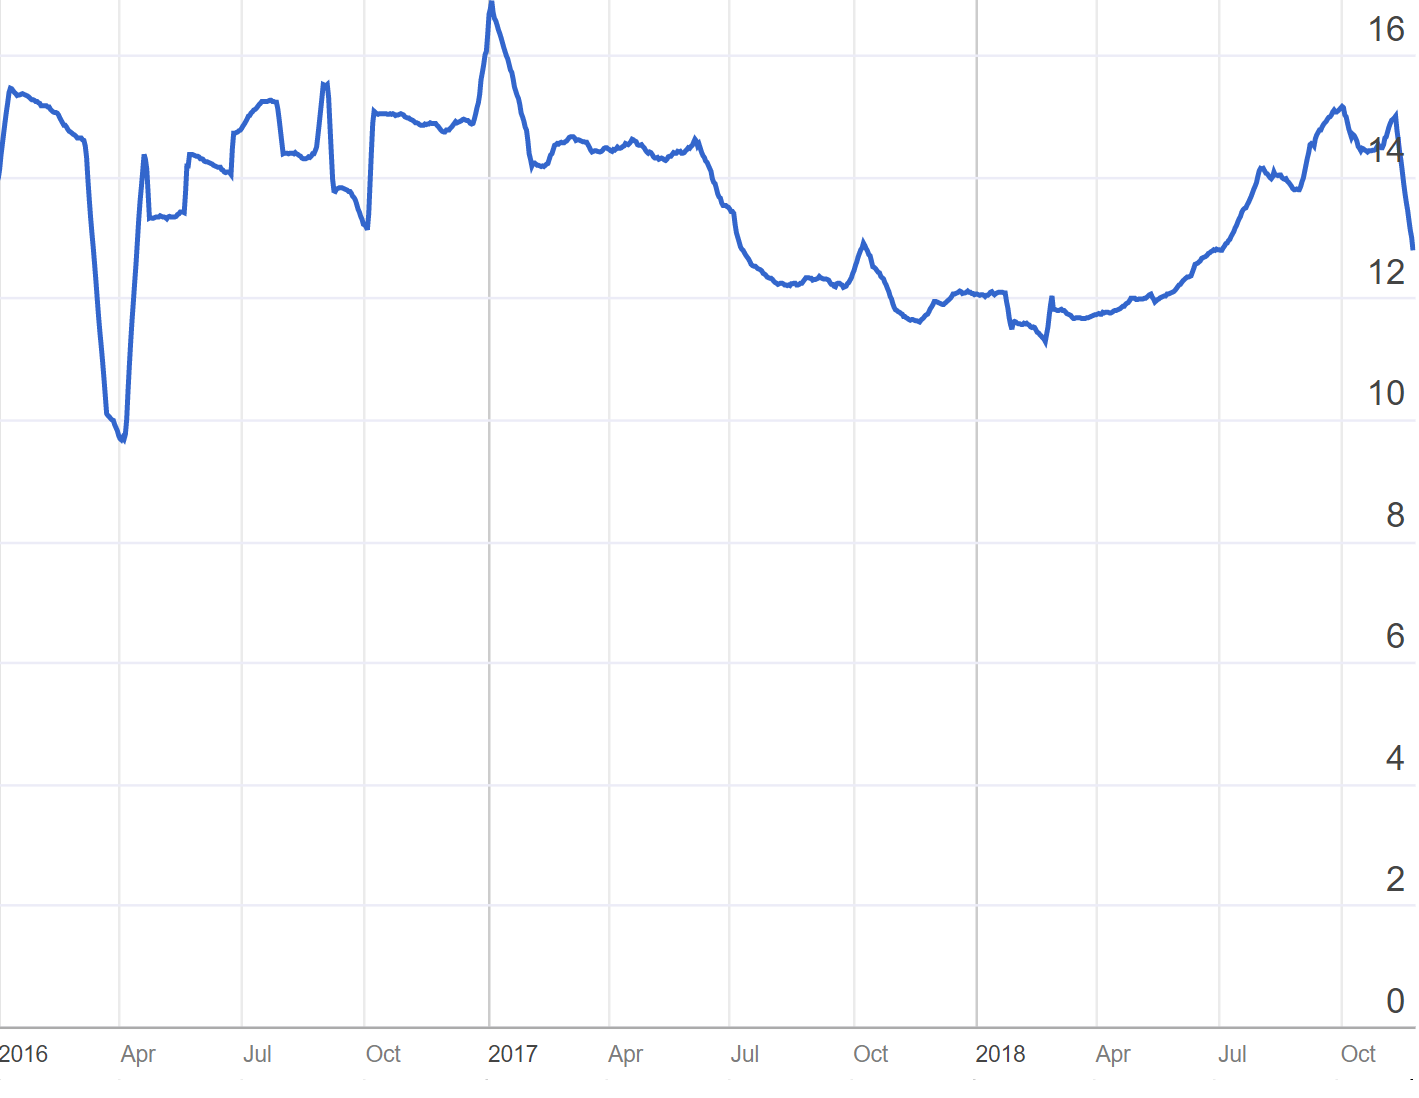
\includegraphics[width=0.95\linewidth]{apnic.png}
    \caption{APNIC estimate of the percentage of global DNS resolvers (Google
    PDNS as well as local resolvers) performing DNSSEC validation from October
    2013 to December 2018. The five year trend is positive.}\label{fig:apnic}
\end{figure*}

The proof-of-concept \DNSSYS{} implementation is only secure if the
corresponding DNS zone is secure, \ie it is protected by DNSSEC. As detailed in
\figref{apnic}, DNSSEC adoption rate---which has increased dramatically since
the first production root zone was signed in 2010~\cite{Cloudflare, APNIC}---is
decidedly variable and slow to rise. Only around 3\% of Fortune 1000 and 9\% of
university domains have properly deployed DNSSEC~\cite{NIST-IPv6}, and the
number of DNS resolvers validating DNSSEC replies currently sits at
approximately 12-14\%~\cite{APNIC}.

While this could be happening for a variety of reasons~\cite{DNSSEC-is-hard-1,
DNSSEC-is-hard-2, DNSSEC-is-hard-3, DNSSEC-is-hard-4, DNSSEC-is-hard-5}, slow
growth is certainly not outside of the norm for global protocol deployments that
are perceived as ``nice to have'' rather than ``business critical''. For
instance: the adoption rate of IPv6, proposed nearly 25 years ago, is similarly
slow to rise. Globally, when measured as the availability of IPv6 connectivity
among users accessing any Google service, it rests at approximately
21\%~\cite{Google-IPv6}, with only 2\% of Fortune 1000 and 3\% of university
domains being IPv6-enabled~\cite{NIST-IPv6}; we note that this is the case
despite IANA and all RIRs having entered the final stage of virtual IPv4
address space exhaustion as of 2018~\cite{APNIC-exhaustion} while the number of
internet-connected devices continues its upward climb~\cite{Cisco}.

With that said, if we assume the user has installed the \DNSSYS{} extension,
slow adoption of DNSSEC globally would in no way impact an individual entity's
ability to adopt and immediately benefit from \DNSSYS{}. We consider this a key
feature of the approach. Those entities that consider their resources' integrity
to be business critical do not have to wait for DNSSEC to be adopted globally.
Any well-configured DNSSEC-protected zone can opt-in to providing the resource
records \DNSSYS{} expects, including a strict mode record, offering power users
verifiable resources while remaining completely transparent to everyone else.
Otherwise, users receiving resources from an entity that is not yet DNSSEC
capable (and so they do not support \DNSSYS{}) will not experience any
interruption in their user experience whether they have a \DNSSYS{}-capable
browser or not.

\subsubsection{DNS-Specific Protocol Limitations}

Clearly, \DNSSYS{} relies on DNS. However, DNS~\cite{DNS1} was not originally
designed to transport or store relatively large amounts of data, though this has
been addressed with EDNS0~\cite{EDNS}. The checksums stored in DNS should not be
much longer than 128 bytes or the output of the SHA512 function. Regardless, DNS
resource record extensions exist that store much more than 128 bytes of
data~\cite{CERT, IPSECKEY, DANE3, DANE1}.

Several working groups are considering DNS as a storage medium for
checksums/hash output as well, such as securitytxt~\cite{draft-sectxt}. A widely
deployed example of DNS ``TXT'' resource records being used this way is SPF and
DKIM~\cite{DKIM}. We are unaware of any practical limitation on the number of
resource records a DNS zone file can support~\cite{DNS1}, hence any
considerations regarding zone file size and/or ceilings on the number of TXT
records in a single zone are at the sole discretion of the implementing entity.

Additionally, \DNSSYS{} does not add to the danger of amplification and other
reflection attacks on DNS; these are generic DNS issues addressable at other
layers of the protocol.

\subsubsection{DHT-Specific Limitations}

Unlike DNS, an entity seeking to leverage a Distributed Hash Table (DHT) may not
have the benefit of being able to rely on a high availability distributed
authenticated backend that is already established, is well-tested, and exists
globally like DNS. Such an entity would have to either maintain their own
network of DHT nodes, which can incur significant cost if such a network was not
already deployed, or piggy back off an open authenticated network, as was done
with the case with our proof-of-concept \DHTSYS{} implementation.

These reasons make DNS with DNSSEC more appealing as an authenticated backend in
comparison. Regardless, we provide \DHTSYS{} to demonstrate the utility and
flexibility of the \SYSTEM{} approach.

\subsubsection{Limitations of a Chrome Extension}

Our current JavaScript proof-of-concept implementations, as Chrome extensions,
are not allowed to touch the resource files downloaded by Chrome and so cannot
prevent a potentially-malicious resource from being executed by the end user---a
feature Chrome/Chromium reserves for its own internal use. The Chrome
\textit{app} API~\cite{AppAPI} might have been of assistance as it allowed for
some limited filesystem traversal via a now deprecated native app API; there is
also a non-standard HTML5/WebExtensions FileSystem API that would provide
similar functionality were it to be widely considered~\cite{deadSpec}.

While still effective, \DNSSYS{} and \DHTSYS{} would be even more effective as
browser extensions if Chrome/Chromium or the WebExtensions API allowed for an
explicit \texttt{onComplete} event hook in the downloads API. This hook would
fire immediately before a file download completed and the file became
executable, \ie had its \texttt{.crdownload} or \texttt{.download} extension
removed. The hook would consume a \texttt{Promise}/\texttt{AsyncFunction} that
kept the download in its non-complete state until said \texttt{Promise}
completed. This protocol would allow the extensions' background pages to do
something like alter the download's \texttt{DangerType} property and alert the
end user to the dangerous download naturally. These modifications would have the
advantage of communicating intent through the browser's familiar UI and
preventing the potentially-malicious download from becoming immediately
executable. Unfortunately, the closest the Chrome/WebExtensions API comes to
allowing \texttt{DangerType} mutations is the \texttt{acceptDanger} method on
the downloads API, but it is not suitable for use with \DNSSYS{} as a background
page based extension.

While nice to have, we stress that none of the aforesaid functionality is
critical to the ability of our implementations to more effectively mitigate SCA
risk than checksums and other solutions (cf. \secref{evaluation}).

\subsection{Future Work}

\subsubsection{Merkle Trees and Early Resource Validation}

Using Merkle trees~\cite{Merkle} instead of pure cryptographic hashing functions
for resource validation would enable partial verification of large files. For
example, suppose we are downloading a 10TiB resource and it is compromised. By
calculating a Merkle tree beforehand, we do not have to wait for the resource to
finish downloading before we render a failing judgment. This partial
verification has the potential to save the user a significant amount of time,
though using Merkle trees for resource integrity validation over the internet is
decidedly not-trivial~\cite{Merkle-HTTP}.

For a production example of Merkle tree based resource integrity validation, we
can look to the so-called \emph{Tiger tree hash}~\cite{TTH, Merkle} (TTH)
construction. The TTH, a Merkle tree implementation, is built on the Tiger
cryptographic hashing function. Merkle trees and TTHs are well-studied and
widely deployed constructions capable of supporting ``partial verification'' of
resources as they are downloaded. Tiger tree hashes in particular are popular
among several large P2P file sharing applications such as WireShare
(LimeWire)~\cite{LimeWire}. Of course, a solution need not be tightly coupled to
the Tiger cryptographic hashing function. The high-speed BLAKE2, SHA2, or SHA3
cryptographic hashing functions would perform just as well, if not better.

\subsubsection{URNs for Wider Compatibility}

The goal of Resource Identifiers (RI) and Non-Authoritative Checksums (NAC) is
very similar to that of Uniform Resource Names (URN). It may make sense to
replace the mapping between NACs/RIs and Authoritative Checksums with purely
URN-based DNS lookups that return specially formatted TXT records upon success.
This would further simplify the deployment process for service administrators
since DNS updates would be based upon the resource's contents instead of both
its contents \textit{and where it is located physically on a distribution
system}. It may also allow for additional confirmation methods of the identical
resources in different domains and in different locations.

We did not create a URN-based scheme in our initial approach due to a new URN
scheme requiring the registration of a unique identifier with the Internet
Assigned Numbers Authority. Going forward, we can potentially adopt a URN scheme
that already exists, such as Magnet links~\cite{MagnetLinks} or the informal
IETF draft for hash-based URN namespaces~\cite{draft-URN}. URNs would allow
\DNSSYS{} and \DHTSYS{} to be much more flexible in how they map resources to
Authoritative Checksums, \ie our proof-of-concept implementations would be able
to handle mirrors and CDNs that may mangle resource path.

\section{Conclusion} \label{sec:conclusion}

Downloading resources over the internet is indeed a risky endeavor. Resource
integrity attacks, and Supply Chain Attacks more broadly, are becoming more
frequent and their impact more widely felt. This paper shows that the de facto
standard for addressing resource integrity risk---the use of \emph{checksums}
coupled with a secure transport layer---is an insufficient and often ineffective
solution. We propose a novel resource validation approach meant as a complete
replacement for checksum based approaches: \SYSTEM{}, which automates the
tedious parts of verification to eliminate user apathy while leveraging
highly-available authenticated distributed systems to ensure resources and
checksums are not co-hosted. Further, we demonstrate the effectiveness and
practicality of our approach versus resource integrity attacks in a real-world
system.

The results of our evaluation show that our approach is more effective than
checksums and other attempts at mitigating resource integrity attacks
against arbitrary resources on the internet. Further, we show \DNSSYS{} is
capable of detecting a wide variety of real-world integrity errors,
significantly raising the bar for the attacker. \DNSSYS{}, as it is backed by
DNS, is immediately deployable at scale for entities that secure their DNS
zone(s) with DNSSEC.

\section{Availability} \label{sec:availability}

We make our DNS\footnote{DNSCHK: \texttt{https://tinyurl.com/dnschk-actual}} and
DHT\footnote{DHTCHK: \texttt{https://tinyurl.com/dhtchk-actual}}
proof-of-concept implementations of HASCHK available to the community open
source so that others can extend it or compare to it. Our hope is that this work
motivates further exploration of resource integrity and other SCA attack
mitigation strategies.

We also make publicly available for your consideration our testing environment:
a patched HotCRP instance\footnote{HotCRP Testbed:
\texttt{https://tinyurl.com/dnschk-hotcrp}}.


\clearpage
\printbibliography
\end{document}
